\section{Nichtlineare Probleme}
\label{sec-5}

Wir diskutieren RB-Ansätze für nichtlineare Probleme anhand von ``quadratischen'' Nichtlinearitäten, Kommentare zur Verallgemeinerung folgen am Ende des Kapitels.

\begin{defn}[Nichtlineares volles Problem $\prob$]
	Sei $X$ Hilbertraum, $\mu \in \p$ gesucht ist $u(\mu) \in X$, $s(\mu) \in \R$ als Lösung von
	\begin{align*}
		a(u,u,v;\mu) + b(u,v;\mu) &= f(v;\mu) \quad \forall v \in X\\
		s(\mu) &= l(u(\mu);\mu)
	\end{align*}
	mit $a$, $b$, $f$, $l$ stetige parametrische Tri-/Bi-/Linearformen.
\end{defn}

\begin{bem}[Wohlgestelltheit] \beginwithlistbem
	\begin{itemize}
		\item Existenz und Eindeutigkeit im Allgemeinen unklar: Mehrere oder keine Lösung möglich.
		\item Lokale Existenz und Eindeutigkeit von $\prob$ wird später a-posteriori nach erfolgreicher RB-Approximation möglich sein.
	\end{itemize}
\end{bem}

\subsubsection*{Annahmen:}
\begin{itemize}
	\item Seien $a$, $b$, $f$, $l$ stetig mit Stetigkeitskonstanten $\gamma_a(\mu)$, $\gamma_b(\mu)$, $\gamma_f(\mu)$, $\gamma_l(\mu)$ und separierbar parametrisch.
	\item Seit $a$ symmetrisch bzgl.\ ersten beiden Argumenten: $a(u,v,\pdot;\mu) = a(v,u,\pdot;\mu)$
	\item Lokale Wohlgestelltheit der Linearisierung:

		Für alle $\mu \in \p$ existiert $\gamma_u \in \R^+ \cup \set{\infty}$, sodass $\forall u \in B(0,\gamma_u) \subset X$ und alle $g \in X'$ die Gleichung
		\begin{equation}
			2a(u,h,\pdot;\mu) + b(h,\pdot;\mu) = g(\pdot)
			\label{eq:5.1}
		\end{equation}
		eine eindeutige Lösung $h \in X$ besitzt mit
		\[
			\norm{h} \leq \frac{1}{\beta(\mu)} \norm{g}_{X'}
		\]
		mit geeignetem Stabilitätsfaktor $\beta(\mu) > 0$.
\end{itemize}

\subsubsection*{Referenzen:}
\begin{itemize}
	\item \,[VPP03]: Veroy, Prud'homme, Patera: Reduced-basis approximation of the viscous Burgers equation: rigorous a posteriori error bounds. C. R. Acad. Sci. Paris, Series I, 337 : 619-624, 2003.
	\item \,[VPRP03]: Veroy, Prud'homme, Rovas, Patera: A posteriori error bounds for reduced-basis approximation of parametrized noncoercive and nonlinear elliptic partial differential equations. In Proc. 16th AIAA computational fluid dynamics conference, 2003, Paper 2003.3847.
\end{itemize}

\subsubsection*{Beispiele:}
\begin{enumerate}[a)]
	\item Poisson-Gleichung mit nichtlinearem Reaktionsterm: gesucht $u \in H_0^1(\Omega) = X$ mit
		\begin{align*}
			-\mu_1 \Delta u + \mu_2 u^2 &= q &\text{in } \Omega,\; \mu_1, \mu_2 > 0\\
			u &= 0 & \text{auf } \partial\Omega
		\end{align*}
		Schwache Form:
		\[
			\underbrace{\mu_1 \int_\Omega \nabla u \cdot \nabla v}_{b(u,v;\mu)} + \underbrace{\mu_2 \int_\Omega u^2 v}_{a(u,u,v;\mu)} = \underbrace{\int_\Omega q v}_{f(v;\mu)} \quad \forall v \in X
		\]
		Für $\Omega \subset \R$, $q \in L^2(\Omega)$ sind (Multi-)Linearformen stetig (via $H_0^1 \to L^4$ stetig).
	\item Viskose Burgers-Gleichung
		\begin{align*}
			-\mu_1 \Delta u + \nabla(\mu_2 u^2) &= q &\text{in } \Omega\\
			u &= 0 & \text{auf } \partial\Omega
		\end{align*}
		Schwache Form:
		\[
			\mu_1 \int_\Omega \nabla u \cdot \nabla v \underbrace{- \mu_2 \int_\Omega u^2 \nabla v}_{a(u,u,v;\mu)} = \int_\Omega q v \quad \forall v \in X
		\]
		Quadratische Nichtlinearität ist ähnlich zu inkompressiblen Navier-Stokes-Gleichungen in mehreren Raumdimensionen.
		Bei Burgers-Gleichung erwartet man also ähnliche Effekte/Probleme wie bei ``echten'' Strömungen.
\end{enumerate}

\subsection*{Numerische Lösung von $\prob$}

\begin{itemize}
	\item Mit $F(u;\mu) := a(u,u,\pdot;\mu) + b(u,\pdot;\mu) - f(\pdot;\mu) \in X'$ lautet Bedingung für $u(\mu)$ einfach $F(u(\mu);\mu) = 0$, also Nullstellensuche.
		Numerische Behandlung mit Newton-Schema möglich.
	\item Richtungsableitungen: $\forall u,h \in X$ gilt
		\begin{align*}
			DF|_u(h) &= \lim_{\delta \to 0} \frac{F(u + \delta h)-F(u)}{\delta}, \quad DF|_u : X \to X'\\
			F(u+\delta h)-F(u) &= a(u+\delta h, u + \delta h,\pdot) - a(u,u,\pdot)\\
			&\quad + b(u+\delta h,\pdot)-b(u,\pdot)+f(\pdot)-f(\pdot)\\
			&= 2 \delta a(u,h,\pdot)+\delta^2 a(h,h,\pdot)+\delta b(h,\pdot)\\
			\Rightarrow \; DF|_u(h) &= 2a(u,h,\pdot)+b(h,\pdot)
		\end{align*}
	\item Newton-Schleife:
		\begin{itemize}
			\item Wähle $u^0 \in X$
			\item Wiederhole:

				\quad Bestimme $h^k$ als Lösung von $DF|_{u^k}(h^k) = -F(u^k)$:
				\[
					2a(u^k,h^k,v)+b(h^k,v) = -a(u^k,u^k,v)-b(u^k,v)+f(v) \quad \forall v \in X
				\]
				\quad Setze $u^{k+1} := u^k + h^k$

				bis $\norm{u^{k+1}-u^k} < \epsilon_{tol}$
			\item Falls Newton-Verfahren konvergiert $\Rightarrow$ Existenz einer Lösung.
		\end{itemize}
\end{itemize}

\begin{defn}[Reduziertes nichtlineares Problem $\rprob$] \label{5.2}
	Sei $X_N \subset X$ RB-Raum, $\mu \in \p$. Gesucht ist $u_N(\mu) \in X_N$, $s_N(\mu) \in \R$ mit
	\begin{align*}
		a(u_N,u_N,v;\mu)+b(u_N,v;\mu)&=f(v;\mu)\\
		s_N(\mu)&=l(u_N)
	\end{align*}
\end{defn}

\begin{bem} \beginwithlistbem
	\begin{itemize}
		\item $\rprob$ ist also äquivalent zu $F_N(u_N(\mu))=0$ für entsprechendes $F_N : X_N \to (X_N)'$ mit $F_N(u):=F(u)|_{X_N}$ $\forall u \in X_N$.
		\item Newton-Verfahren liefert wieder eine Sequenz $\seq{u_N^k}_k \subset X_N$.
			Falls diese konvergiert, haben wir (lokale) Lösung von $\rprob$.
	\end{itemize}
\end{bem}

\subsubsection*{Offline-Online-Zerlegung:}
Sei $X_N = \spn\set{\phi_1,\ldots,\phi_N}$

Offline:
\begin{align*}
	\ubar f_N^q &:= \seq{f^q(\phi_i)}_{i=1}^N, & \ubar l_N^q &:= \seq{l^q{\phi_i}}_{i=1}^N\\
	\ubar B_N^q &:= \seq{b^q(\phi_j,\phi_i)}_{i,j=1}^N, & \ubar K_N &:= \seq{\dotp{\phi_i}{\phi_j}}_{i,j=1}^N\\
	\ubar A_N^q &:= \seq{a^q(\phi_i,\phi_j,\phi_k)}_{i,j,k=1}^N \in \R^{N \times N \times N}
\end{align*}

Online:
\begin{itemize}
	\item Setze $\mu \in \p$
	\item Setze $\ubar A_N(\mu) := \sum_{q=1}^{Q_a} \Theta_a^q(\mu) \ubar A_N^q$, analog $\ubar f_N(\mu)$, $\ubar l_N(\mu)$, $\ubar B_N(\mu)$
	\item Wähle $\ubar u_N^0 = \seq{u_{N,i}^0}_{i=1}^N \in \R^N$
	\item Wiederhole:
		\begin{itemize}
			\item Bestimme $\ubar h_N^k \in \R^N$ als Lösung von
				\[
					\left( 2\sum_{n=1}^N (\ubar A_N)_{n,:,:} u_{N,n}^k + \ubar B_N \right) \ubar h_N^k = -\sum_{n,m=1}^N (\ubar A_N)_{n,m,:} u_{N,n}^k - \ubar B_N \ubar u_N^k + \ubar f_N
				\]
			\item $\ubar u_N^{k+1} := \ubar u_N^k + \ubar h_N^k$
		\end{itemize}
	\item Bis $(\ubar u_N^{k+1} - \ubar u_N^k) \ubar K_N (\ubar u_N^{k+1} - \ubar u_N^k) < \epsilon_{tol}^2$
	\item Setze $\ubar u_N := \ubar u_N^{k+1}$, $s_N(\mu) := \ubar l_N^T \ubar u_N$
\end{itemize}

\begin{bem}
	Komplexität $\O(Q_a N^3)$ für Speichern und Linearkombinieren von $A_N(\mu)$ aus Komponenten ist erheblich.
\end{bem}

\subsubsection*{Lösungstheorie für $\prob$}

\begin{satz}[Inversion gestörter Operator] \label{5.3}
	Seien $A$, $B \in L(X,Y)$, $A$ invertierbar.
	Falls $\norm{A^{-1}B}_{X;X} := \sup_{x \neq 0} \frac{\norm{A^{-1}Bx}_X}{\norm{x}_X} < 1$, so ist $A + B$ invertierbar und
	\[
		\norm{(A+B)^{-1}}_{Y;X} \leq \frac{1}{1-\norm{A^{-1}B}_{X;X}} \norm{A^{-1}}_{Y;X}
	\]

	\begin{proof}
		Identisch zu Störungssatz für Inversion von Matrizen. $\leadsto$ NLA/Numerik 1.
	\end{proof}
\end{satz}

\begin{satz}[Lokale Existenz und Eindeutigkeit für Nichtlineare Probleme] \label{5.4}
	Sei $G: X \to Y$ eine $C^1$-Abbildung (d.h. $DG$ stetig auf $X$).
	Sei $v \in X$ mit $DG|_v \in L(X,Y)$ Isomorphismus.
	Definiere
	\begin{align*}
		\epsilon &:= \norm{G(v)}_Y\\
		\gamma &:= \norm{(DG|_v)^{-1}}_{Y;X}\\
		L(\alpha) &:= \sup_{x \in \bar B(v, \alpha)} \norm{DG|_v - DG|_x}_{X;Y}
	\end{align*}
	Falls $2 \gamma L(2 \gamma \epsilon) \leq 1$ $\Rightarrow$ existiert eindeutiges $u \in \bar B(v,2\gamma\epsilon)$ mit
	\[
		G(u) = 0
	\]
	und $DG|_u$ invertierbar mit
	\[
		\norm{(DG|_u)^{-1}}_{Y;X} \leq 2\gamma
	\]
	Für alle $x \in \bar B(v,2\gamma\epsilon)$ gilt
	\[
		\norm{x-u}_X \leq 2 \gamma \norm{G(x)}_Y
	\]
\end{satz}

\begin{bem} \beginwithlistbem
	\begin{itemize}
		\item Satz und Beweis aus Theorem 2.1 in

			Caloz, Rappaz: Numerical Analysis For Nonlinear And Bifurcation Problems. In P.G. Ciarlet and J.L. Lions, ``Handbook of Numerical Analysis Vol. V'', Elsevier '97.
		\item Anschauung: Falls $v$ approximative Lösung mit genügend kleinem Residuum und $DG$ lokal invertierbar und $DG$ ändert sich nicht zu start, dann muss Lösung $u$ existieren.
			\begin{figure}[H]
				\centering\small
				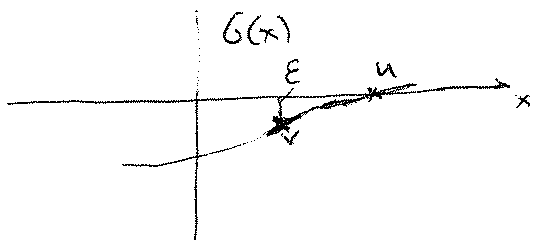
\includegraphics[width = 0.5 \textwidth]{Bilder/existenz-lokale-inverse.png}
			\end{figure}
	\end{itemize}
\end{bem}

\begin{proof}
	Definiere $H : X \to X$
	\[
		H(x) := x - (DG|_v)^{-1} G(x)
	\]
	$u$ Fixpunkt von $H$ $\Leftrightarrow$ $G(u) = 0$.

	Suche also Fixpunkt mit Banach'schem Fixpunktsatz. Sei $x \in \bar B(v,2\gamma\epsilon) =: \bar B$
	\[
		H(x) - v = (DG|_v)^{-1} \left[ DG|_v(x-v)-(G(x)-G(v)) \right] - (DG|_v)^{-1}G(v)
	\]
	Hauptsatz der Differential- und Integralrechnung:
	\[
		G(x)-G(v) = \int_0^1 DG|_{v+t(x-v)}(x-v) \, dt
	\]
	\[
		\Rightarrow \; H(x)-v=(DG|_v)^{-1} \underbrace{\left[ DG|_v(x-v)-\int_0^1 DG|_{v+t(x-v)}(x-v) \, dt \right]}_{\int_0^1 (DG|_v-DG|_{v+t(x-v)})(x-v) \, dt} - (DG|_v)^{-1}G(v)
	\]
	\begin{align} \label{eq:5.2}
		\norm{H(x)-v} &\leq \gamma \int_0^1 \norm{DG|_v - DG|_{v+t(x-v)}}_{X;Y} \, dt \cdot \norm{x-v}_X + \gamma \cdot \epsilon\\
		&\leq \gamma \cdot \underbrace{L(2\gamma \epsilon) \cdot 2 \gamma}_{\leq 1} \epsilon + \gamma \epsilon \leq 2\gamma \epsilon \notag
	\end{align}
	$\Rightarrow$ $H(x) \in \bar B$ also $H(\bar B) \subseteq \bar B$ Selbstabbildung von $\bar B$ auf $\bar B$.
	Seien $x$, $x' \in \bar B$
	\begin{align*}
		H(x)-H(x') &= x-(DG|_v)^{-1}G(x)-x'+(DG|_v)^{-1}G(x')\\
		&= x-x'-(DG|_v)^{-1}(G(x)-G(x'))\\
		&= (DG|_v)^{-1} DG|_v(x-x')-(DG|_v)^{-1} \int_0^1 DG|_{x'+t(x-x')}(x-x') \, dt\\
		&= (DG|_v)^{-1} \int_0^1 (DG|_v-DG|_{x'+t(x-x')})(x-x') \, dt \tag{5.2'} \label{eq:5.2'}
	\end{align*}
	\[
		\Rightarrow \; \norm{H(x)-H(x')} \leq \gamma L(2\gamma\epsilon) \norm{x-x'} \leq \frac{1}{2} \norm{x-x'}
	\]
	also $H$ Kontraktion auf $\bar B$.
	$\stackrel{\text{BFPS}}{\Rightarrow}$ es existiert eindeutiger Fixpunkt $u \in \bar B$.

	Mit Störungssatz \ref{5.3} ist $DG|_u$ invertierbar:
	\[
		DG|_u = \underbrace{DG|_v}_{''A''} + \underbrace{(DG|_u-DG|_v)}_{''B''}
	\]
	und
	\[
		\norm{(DG|_v)^{-1}(DG|_u-DG|_v)}_{X;X} \leq \gamma L(2\gamma\epsilon) \leq \frac{1}{2}
	\]
	\[
		\Rightarrow \; \norm{(DG|_u)^{-1}}_{Y;X} \leq \frac{1}{1-\frac{1}{2}}\gamma = 2\gamma
	\]
	\begin{align*}
		u-x &= H(u)-x \\
		&= u-(DG|_v)^{-1}G(u)-x\\
		&=(DG|_v)^{-1}(DG|_v)(u-x)-(DG|_v)^{-1}\overbrace{\left( G(x)+\int_0^1 DG|_{x+t(u-x)}(u-x) \, dt \right)}^{= G(u)}\\
		&=(DG|_v)^{-1} \left[-G(x)-\int_0^1 (DG|_v-DG|_{x+t(u-x)})(u-x) \, dt \right]
	\end{align*}
	\[
		\Rightarrow \; \norm{u-x} \leq \gamma [\norm{G(x)}+L(2\gamma\epsilon)\norm{u-x}]
	\]
	\[
		\Rightarrow \; \underbrace{(1-\overbrace{\gamma L(2\gamma\epsilon)}^{\leq \frac{1}{2}}) \norm{u-x}} \leq \gamma \norm{G(x)} \quad \Rightarrow \quad \norm{u-x} \leq 2 \gamma \norm{G(x)}
	\]
\end{proof}

Dieser Satz ist für unser $\prob$ anwendbar wegen der Annahme der Wohlgestelltheit der Linearisierungen \eqref{eq:5.1}:

\begin{kor}[Lokale Existenz und Eindeutigkeit für $\prob$] \label{5.5}
	Sei $u_N(\mu)$ eine Lösung für $\rprob$.
	Setze duale Norm des Residuums
	\begin{equation}
		\epsilon := \norm{F(u_N)}_{X'} = \norm{a(u_N,u_N,\pdot;\mu)+b(u_N,\pdot)-f(\pdot)}_{X'}
		\label{eq:5.3}
	\end{equation}
	und verallgemeinerte inf-sup Konstante
	\[
		\beta_{u_N}(\mu) := \norm{(DF|_{u_N})^{-1}}_{X';X}^{-1} \geq \beta(\mu) > 0
	\]
	und $L_{DF} := 2\gamma_a \in \R$ Lipschitz-Konstante von $DF$ bzgl.\ $v$: $\norm{DF|_u-DF|_v} \leq L_{DF} \norm{u-v}$.
	Falls
	\[
		\frac{8\epsilon\gamma_a}{\beta_{u_N}^2(\mu)} \leq 1
	\]
	so existiert eindeutige $u \in B(u_N,\frac{2\epsilon}{\beta_{u_N}})$ Lösung von $\prob$.

	\begin{proof}
		$L_{DF} = 2\gamma_a$ ist tatsächlich Lipschitz-Konstante, denn
		\begin{align*}
			(DF|_u-DF|_v)(h)(w) &= |2a(u,h,w)+b(h,w)-2a(v,h,w)-b(h,w)|\\
			&= |2a(u-v,h,w)| \leq 2\gamma_a \norm{u-v}\norm{h}\norm{w}\\
			\Rightarrow \; \norm{DF|_u-DF|_v}_{X,X'} &= \sup_{h\in X} \sup_{w\in X} \frac{|(DF|_u-DF|_v)(h)(w)|}{\norm{h}\norm{w}} \leq 2\gamma_a \norm{u-v}
		\end{align*}
		Überprüfe Bedingung von Satz \ref{5.4} mit $G=F$, $v=u_N$:

		$F$ ist $C^1$ Abbildung ($DF$ stetig auf $X$)

		$DF|_{u_N} \in L(X,X')$ Isomorphismus nach Annahme.
		\begin{align*}
			\epsilon &\;= \norm{F(u_N)}_{X'}\\
			\gamma &:= \norm{(DF|_{u_N})^{-1}}_{X';X} = \frac{1}{\beta_{u_N}}\\
			L(\alpha) &:= \sup_{x\in\bar B(u_N,\alpha)} \norm{DF|_{u_N}-DF|_x}_{X;X'}\\
			&\;\leq \sup_{x\in\bar B(u_N,\alpha)} L_{DF} \norm{u_N-x} = L_{DF} \alpha = 2\gamma_a \alpha\\
			2\gamma L(2\gamma\epsilon) &\;\leq 2\gamma L_{DF} \cdot 2\gamma\epsilon = \frac{4L_{DF}\epsilon}{\beta_{u_N}^2} = \frac{8\epsilon\gamma_a}{\beta_{u_N}^2} \leq 1
		\end{align*}
		$\stackrel{\ref{5.4}}{\Rightarrow}$ existiert eindeutige $u \in \bar B(u_N,2\gamma\epsilon)$ Lösung von $F(u)=0$.
	\end{proof}
\end{kor}

\begin{bem}
	Mit untere Schranke $0 < \beta_{LB}(\mu) \leq \beta_{u_N}(\mu)$ hat man mit obigem also auch Fehlerschätzer $\norm{u-u_N} \leq \frac{2\epsilon}{\beta_{LB}}$.
	Dies lässt sich jedoch noch wesentlich verbessern und Effektivitäten beweisen:
\end{bem}

\begin{satz}[A-posteriori Fehlerschätzer und Effektivitätsschranke] \label{5.6}
	Sei $u_N$ Lösung von $\rprob$ aus Definition \ref{5.2} und $\beta_{LB} \leq \beta_{u_N}$, $\epsilon$ aus \eqref{eq:5.3} duale Norm des Residuums, $\epsilon := \norm{F(u_N;\mu)}_{X'}$.
	Sei
	\[
		\tau := \frac{4\epsilon L_{DF}}{\beta_{LB}^2} = \frac{8 \epsilon\gamma_a}{\beta_{LB}^2} \leq 1
	\]
	und $u$ eindeutige Lösung von $\prob$ in $B(u_N,\frac{2\epsilon}{\beta_{u_N}})$ gemäß Korollar \ref{5.5}. Dann gilt
	\[
		\norm{u-u_N} \leq \Delta_N := \frac{\beta_{LB}}{2 L_{DF}} (1-\sqrt{1-\tau})
	\]
	\[
		\eta_N := \frac{\Delta_N}{\norm{u-u_N}} \leq 4 \frac{\gamma_{DF}(u_N)}{\beta_{LB}}
	\]
	mit $L_{DF} = 2\gamma_a$ und
	\[
		\gamma_{DF} := 2\gamma_a \norm{u_N}+\gamma_b \geq \norm{DF|_{u_N}}_{X;X'}
	\]
\end{satz}

\begin{bem} \beginwithlistbem
	\begin{itemize}
		\item $\beta_{LB}$ im Zähler sieht zunächst seltsam aus. Weil $\tau \in [0,1]$ ist $(1-\sqrt{1-\tau}) \in [0,1]$, also insbesondere $\sqrt{(\pdot)}$ wohldefiniert und
			\begin{equation} \label{eq:5.4}
				\Delta_N \leq \frac{\beta_{LB}}{2 L_{DF}} \tau = \frac{\beta_{LB}}{2 L_{DF}} \cdot \frac{4 \epsilon L_{DF}}{\beta_{LB}^2} = \frac{2 \epsilon}{\beta_{LB}}
			\end{equation}
			Also gewohnte Struktur: Residuum durch Stabilitätskonstante, jedoch Faktor 2.
	\end{itemize}
\end{bem}

\begin{proof}
	Ähnlich zu \ref{5.4}, statt festem Radius betrachte Kugel mit variablem Radius $\alpha$.
	Weil $DF$ Lipschitz-stetig, ist $H(x)= x-(DF|_{u_N})^{-1} H(x)$ Kontraktion auf $B(u_N,\alpha)$ falls $\alpha \leq \frac{\beta_{LB}}{2 L_{DF}} = \frac{\beta_{LB}}{4 \gamma_a} =: \hat\alpha$:\\ \\
	Für $x$, $x' \in B(u_N,\alpha)$ ist mit \eqref{eq:5.2'}
	\[
		\norm{H(x)-H(x')} \stackrel{\eqref{eq:5.2'}}{\leq} \overbrace{\gamma}^{\leq \frac{1}{\beta_{LB}}} \underbrace{L(\alpha)}_{\mathclap{\leq L_{DF} \alpha \leq L_{DF} \cdot \frac{\beta_{LB}}{2 L_{DF}}}} \leq \frac{1}{\beta_{LB}} \cdot L_{DF} \cdot \frac{\beta_{LB}}{2 L_{DF}} \norm{x-x'} = \frac{1}{2} \norm{x-x'}
	\]
	Suche nun Bedingung für $\alpha$ sodass $H$ Selbstabbildung auf $B(u_N,\alpha)$. Mit \eqref{eq:5.2} folgt für $x \in B(u_N,\alpha)$
	\begin{align*}
		\norm{H(x)-u_N} &\leq \underbrace{\gamma}_{\leq \frac{1}{\beta_{LB}}} \left( \int_0^1 \norm{DF|_{u_N} - DF|_{u_N+t(x-u_N)}}_{X;X'} \right) \underbrace{\norm{x-u_N}}_{\leq \alpha} + \gamma \cdot \epsilon\\
		&\leq \frac{1}{\beta_{LB}} L_{DF} \alpha^2 + \frac{1}{\beta_{LB}} \epsilon
	\end{align*}
	Falls also
	\begin{equation} \label{eq:5.5}
		\frac{L_{DF}}{\beta_{LB}} \alpha^2 + \frac{\epsilon}{\beta_{LB}} \leq \alpha
	\end{equation}
	so ist $H$ Selbstabbildung.
	\begin{align*}
		\eqref{eq:5.5} \quad \Leftrightarrow \quad &\alpha^2 - \frac{\beta_{LB}}{L_{DF}} \alpha + \frac{\beta_{LB}}{L_{DF}} \cdot \frac{\epsilon}{\beta_{LB}} \leq 0\\
		\Leftrightarrow \quad &\alpha \in [\alpha_-,\alpha_+] \text{ mit } \alpha_\pm := \frac{\beta_{LB}}{2 L_{DF}} \pm \sqrt{\frac{\beta_{LB}^2}{4L_{DF}^2}-\frac{\epsilon}{L_{DF}}}\\
		&\alpha_\pm = \hat\alpha \left( 1 \pm \sqrt{1-\frac{\epsilon}{L_{DF} \hat\alpha^2}} \right) = \hat\alpha ( 1 \pm \sqrt{1-\tau})
	\end{align*}
	weil
	\[
		\frac{\epsilon}{L_{DF} \hat\alpha^2} = \frac{\epsilon}{L_{DF}} \cdot \frac{4 L_{DF}^2}{\beta_{LB}^2} = \frac{4 L_{DF}}{\beta_{LB}^2} \epsilon = \tau \leq 1
	\]
	also $\alpha_\pm$ wohldefiniert.\\
	\\
	Für $\alpha \in [\alpha,\hat\alpha]$ ist $H$ Selbstabbildung und Kontraktion.
	Für kleinstes $\alpha = \alpha_-$ erhalte beste Schranke, also ex.\ $u \in B(u_N,\alpha_-)$ mit
	\[
		\norm{u-u_N} \leq u_N = \alpha_-
	\]
	Für Effektivitätsschranke setze $e := u-u_N$.
	Sei $v_r \in X$ Riesz-Repräsentant des Residuums
	\[
		\dotp{v_r,v} = F(u_N)(v)
	\]
	Benötigt Fehler-Residuums-Beziehung für quadratisches Problem
	\begin{align*}
		F(u_N) &= a(u_N,u_N,\pdot) - b(u_N,\pdot) - \underbrace{f(\pdot)}_{\mathclap{= a(u,u,\pdot)-b(u,\pdot)}}\\
		&= 2 a(u_N,u_N,\pdot) - 2 a(u_N,u,\pdot) - a(u_N,u_N,\pdot)\\
		&\qquad + 2 a(u_N,u,\pdot) - a(u,u,\pdot) - b(u-u_N,\pdot)\\
		&= -2 a(u_N,e,\pdot) - b(e,\pdot) - a(e,e,\pdot)\\
		&= -DF|_{u_N}(e) - a(e,e,\pdot)
	\end{align*}
	\begin{align*}
		\Rightarrow \norm{v_r}^2 &= \dotp{v_r,v_r} = F(u_N)(v_r) = -DF|_{u_N}(e)(v_r) - a(e,e,v_r)\\
		&\leq \gamma_{DF}(u_N) \norm{e} \norm{v_r} + \gamma_a \norm{e} \norm{v_r}\\
		\Rightarrow \norm{v_r} &\leq \gamma_{DF}(u_N) \norm{e} + \gamma_a \norm{e}^2
	\end{align*}
	Mit $\norm{v_r} = \epsilon$ und $\Delta_N \stackrel{\eqref{eq:5.4}}{\leq} \frac{2 \epsilon}{\beta_{LB}}$ folgt
	\[
		\Delta_N \leq \frac{2 \norm{v_r}}{\beta_{LB}} \leq \frac{2}{\beta_{LB}} \gamma_{DF} \norm{e} + \frac{2}{\beta_{LB}} \gamma_a \underbrace{\norm{e}^2}_{\leq \Delta_N \cdot \Delta_N}
	\]
	Wegen
	\[
		\frac{2}{\beta_{LB}} \gamma_a \Delta_N \leq \frac{2 \gamma_a}{\beta_{LB}} \cdot \frac{2 \epsilon}{\beta_{LB}} = \frac{4 \gamma_a \epsilon}{\beta_{LB}^2} = \frac{1}{2} \tau \leq \frac{1}{2}
	\]
	folgt
	\[
		\Delta_N \leq \frac{2}{\beta_{LB}} \gamma_{DF} \norm{e} + \frac{1}{2} \Delta_N \quad \Rightarrow \quad \frac{1}{2} \Delta_N \leq \frac{2}{\beta_{LB}} \gamma_{DF} \norm{e}
	\]
	\[
		\Rightarrow \frac{\Delta_N}{\norm{e}} \leq \frac{4 \gamma_{DF}(u_N)}{\beta_{LB}}
	\]
\end{proof}

\begin{bem} \beginwithlistbem
	\begin{itemize}
		\item Lokale Existenz und Eindeutigkeit und Fehlerschranken gilt analog für allgemeinere Nichtlinearitäten $F$, welche Lipschitz-stetige Ableitungen besitzen.
			Nur die Effektivitätsschranke in \ref{5.6} verwendet die Struktur des quadratischen nichtlinearen Problems.
		\item Ausgabe-Fehlerschranken sind einfach möglich analog zu $\Delta_{N,s}$ aus §\ref{sec-3}.
			Auch verbesserte Abschätzung mittels geeigneten dualen Problems ist möglich.
		\item Berechnung von $\beta_{LB}$ durch SCM-ähnliche Techniken möglich, siehe [VPP03].
		\item Falls PDE linear, aber Ausgabe quadratisch nichtlinear, lässt sich ein erweitertes Hilfsproblem formulieren, welche linear, inf-sup-stabil, symmetrisch ist und identische Ausgabe wie Originalproblem mittels geeignetem linearen Ausgabefuntionals liefert.
			$\Rightarrow$ Techniken aus §\ref{sec-3} und §\ref{sec-4} anwendbar.
			Damit z.B.\ Fehlerfunktionale $s(\mu) = \int_\Omega (u(\mu)-u_d)^2$ oder Variationen oder Energien in verschiedenen Versionen behandelbar.\\
			Referenz: [HP07]: ``Reduced basis approximation and a posteriori error estimation for stress intensity factors'', IJNME, 72, 1219-1259, 2007.
		\item Falls PDE polynomiell in $u$ der Ordnung $p$, lässt sich eine $p+1$ Multilinearform-Formulierung der schwachen Form finden und Techniken aus §\ref{sec-5} analog anwenden.
			Problem wird für $p \gg 3$ jedoch die Offline-Online-Zerlegung (...???) weil Komponenten-Tensoren der Stufe $p+1$, also sind Offline Datenmengen und Assemblierungskosten $\O(Q_a N^{p+1})$.
		\item Falls PDE nichtpolynomiell nichtlinear, kann mit Hilfe der EI ein nichtlineares reduziertes Problem formuliert werden.
			Eine Variante ist die Empirische Operatorinterpolation in
			\begin{itemize}
				\item \,[HOR08]: Haasdonk, Ohlberger, Rozza: A Reduced Basis Method for Evolution Schemes with Parameter-Dependent Explicit Operators, ETNA, 32:145-161, 2008.
				\item \,[DHO12]: Drohmann, Haasdonk, Ohlberger: Reduced Basis Approximation for Nonlinear Parametrized Evolution Equations based on Empirical Operator Interpolation, SJSC, 34:A937-A969, 2012.
			\end{itemize}
	\end{itemize}
\end{bem}
